\documentclass{beamer}
\usepackage[UTF8]{ctex}
\usepackage{graphicx}
\usepackage{amsmath,amssymb}
\usepackage{algorithm2e}
\usepackage{tikz}
\usetikzlibrary{shapes,arrows,positioning,decorations.pathmorphing}
\usepackage{hyperref}
\usepackage{booktabs} % 高级表格
\usepackage{multirow} % 跨行表格
\usepackage{pgfplots} % 绘制图表
\pgfplotsset{compat=1.18}

\usetheme{Madrid}
\usecolortheme{default}
\setbeamertemplate{navigation symbols}{}
\setbeamertemplate{caption}[numbered] % 启用图表编号

% 自定义颜色
\definecolor{myblue}{RGB}{30,144,255}
\definecolor{mygreen}{RGB}{50,205,50}
\definecolor{myred}{RGB}{220,20,60} % 用于提示思考的颜色

% config.tex
% 指定 XeLaTeX 编译
%!TeX program = xelatex

%%%%%%%%%%%%%%%%%%%%%%%%%%%%%%%%%%%%%%%%%%%%%%%%%%%%%%%%%%
% 文档类与全局设置
%%%%%%%%%%%%%%%%%%%%%%%%%%%%%%%%%%%%%%%%%%%%%%%%%%%%%%%%%%
\documentclass{beamer}

%tikz包
\usepackage{amsmath, amssymb, xcolor, tikz}
\usetikzlibrary{calc}  % 计算坐标
\usetikzlibrary{backgrounds}  % 背景支持（如果想使用 on background layer）
\usepackage[most]{tcolorbox}
\usepackage{xparse}

%字体设置
\usepackage{fontspec}
\usepackage{xeCJK}
\usepackage{unicode-math}
\usepackage{etoolbox} % 用于开关切换

\newtoggle{fontBlackTheme}
\togglefalse{fontBlackTheme}

\newcommand{\UseBlackFont}{\toggletrue{fontBlackTheme}}
\newcommand{\UseSongFont} { \togglefalse{fontBlackTheme}}

\UseSongFont   % ← 这里启用“宋体+Times New Roman”主题
% 或者 \UseBlackFont ← 启用“黑体+Liberation Sans”主题
\UseBlackFont
%—— 根据开关选择字体 —— 
\iftoggle{fontBlackTheme}{
  % —— 黑体 + Liberation Sans —— 
  % 英文字体
  \setmainfont{Liberation Sans}
  \setsansfont{Liberation Sans}
  \setmonofont{Liberation Mono}
  % 数学字体
  \setmathfont{TeX Gyre Termes Math}
  % 中文黑体
  \setCJKmainfont{Noto Sans CJK SC}
  \setCJKsansfont{Noto Sans CJK SC}
  \setCJKmonofont{Noto Sans CJK SC}
}{
  % —— 宋体 + New Roman 风格 —— 
  % 英文字体
  \setmainfont{Times New Roman}        % 或 TeX Gyre Termes 
  \setsansfont{Times New Roman}         % 可选
  \setmonofont{Times New Roman}         % 可选
  % 数学字体（New Roman 样式）
  \setmathfont{TeX Gyre Termes Math}
  % 中文宋体
  \setCJKmainfont{Noto Serif CJK SC}
  \setCJKsansfont{Noto Serif CJK SC}
  \setCJKmonofont{Noto Serif CJK SC}
}

%%%%%%%%%%%%%%%%%%%%%%%%%%%%%%%%%%%%%%%%%%%%%%%%%%%%%%%%%%
% 图形、色彩与数学设置
%%%%%%%%%%%%%%%%%%%%%%%%%%%%%%%%%%%%%%%%%%%%%%%%%%%%%%%%%%
\usepackage{tikz}
\usepackage[table]{xcolor}    % 表格色块
\usepackage{booktabs}         % 三线表格式
\usepackage{pgfplots}
\pgfplotsset{compat=1.18}

\usepackage{tcolorbox}
\usepackage{amsmath}
\usepackage{xcolor}

\usepackage{unicode-math}
\setmathfont{TeX Gyre Termes Math}
\setbeamercolor{block title}{fg=black,bg=gray!10}
\setbeamerfont{block title}{size=\normalsize,family=\rmfamily}


%%%%%%%%%%%%%%%%%%%%%%%%%%%%%%%%%%%%%%%%%%%%%%%%%%%%%%%%%%
% Beamer 主题与风格设置
%%%%%%%%%%%%%%%%%%%%%%%%%%%%%%%%%%%%%%%%%%%%%%%%%%%%%%%%%%
% 清除默认页眉与 frametitle 模板（后续自定义）
\setbeamertemplate{headline}{}
\setbeamertemplate{frametitle}{}
\setbeamertemplate{itemize item}[circle]

% 内外主题（可根据需求替换）
\useoutertheme[subsection=true]{miniframes} 
\useinnertheme{default}
\usecolortheme{default}

%%%%%%%%%%%%%%%%%%%%%%%%%%%%%%%%%%%%%%%%%%%%%%%%%%%%%%%%%%
% 颜色定义（可自定义调色板）
%%%%%%%%%%%%%%%%%%%%%%%%%%%%%%%%%%%%%%%%%%%%%%%%%%%%%%%%%%
\definecolor{lightblue}{RGB}{70,130,180}
\definecolor{midblue}{RGB}{28,70,130}
\definecolor{darkblue}{RGB}{10,40,80}
\definecolor{myred}{RGB}{150,50,30}
\definecolor{mygreen}{RGB}{45,125,77}
\definecolor{mypurple}{RGB}{120,61,137}
\definecolor{myorange}{RGB}{190,88,32}
\definecolor{myitem}{RGB}{35,35,35}


%%%%%%%%%%%%%%%%%%%%%%%%%%%%%%%%%%%%%%%%%%%%%%%%%%%%%%%%%%
% 导航栏与页眉设置
%%%%%%%%%%%%%%%%%%%%%%%%%%%%%%%%%%%%%%%%%%%%%%%%%%%%%%%%%%
\makeatletter
% 设置顶部导航栏（用于章节、子章节导航）
\setbeamertemplate{headline}{%
  \begin{beamercolorbox}[wd=\paperwidth,ht=2ex,dp=1ex]{section in head/foot}
    \insertsectionnavigationhorizontal{\paperwidth}{}{}%
  \end{beamercolorbox}%
}
\setbeamercolor{section in head/foot}{bg=darkblue, fg=white}
\setbeamercolor{subsection in head/foot}{bg=midblue, fg=white}

% 自定义页眉（仅在非封面页显示 frametitle 和横线，且 frametitle 不为空时才显示）
\setbeamertemplate{headline}{%
  \ifnum\value{framenumber}>1
    \ifx\insertframetitle\@empty
      % 不显示任何内容
    \else
      \begin{tikzpicture}[remember picture,overlay]
        \node[anchor=west, font=\normalsize, text=black, xshift=0.2cm, yshift=-0.4cm]
              at (current page.north west){\insertframetitle};
        \draw[line width=1pt, color=midblue]
              ([yshift=-0.7cm]current page.north west) -- ([yshift=-0.7cm]current page.north east);
      \end{tikzpicture}
    \fi
  \fi
}
\makeatother
%%%%%%%%%%%%%%%%%%%%%%%%%%%%%%%%%%%%%%%%%%%%%%%%%%%%%%%%%%
% 图注样式设置
%%%%%%%%%%%%%%%%%%%%%%%%%%%%%%%%%%%%%%%%%%%%%%%%%%%%%%%%%%
\setbeamerfont{caption}{size=\footnotesize}
\setbeamercolor{caption}{fg=black}
% 此处使用默认字体，确保中文统一为 Noto Sans CJK SC
\setbeamerfont{caption name}{size=\footnotesize}
\setbeamercolor{caption name}{fg=black}
\setbeamertemplate{caption}[numbered]
\renewcommand{\figurename}{图}

%%%%%%%%%%%%%%%%%%%%%%%%%%%%%%%%%%%%%%%%%%%%%%%%%%%%%%%%%%
% 列表样式设置
%%%%%%%%%%%%%%%%%%%%%%%%%%%%%%%%%%%%%%%%%%%%%%%%%%%%%%%%%%
% 自定义无序列表图标，采用 \raisebox 微调图标位置
\newcommand{\useBigCircleItem}{%
  \setbeamertemplate{itemize item}{\raisebox{0.3ex}{\tikz{\draw[myitem, fill=myitem] (0,0) circle (2pt);}}}%
  \setbeamertemplate{itemize subitem}{\raisebox{0.3ex}{\tikz{\draw[myitem, fill=myitem] (0,0) circle (2pt);}}}%
  \setbeamertemplate{itemize subsubitem}{\raisebox{0.3ex}{\tikz{\draw[myitem, fill=myitem] (0,0) circle (2pt);}}}%
}
\newcommand{\useSmallCircleItem}{%
  \setbeamertemplate{itemize item}{\raisebox{0.35ex}{\tikz{\draw[myitem, fill=myitem, opacity=0.8] (0,0) circle (1pt);}}}%
  \setbeamertemplate{itemize subitem}{\raisebox{0.35ex}{\tikz{\draw[myitem, fill=myitem, opacity=0.8] (0,0) circle (1pt);}}}%
  \setbeamertemplate{itemize subsubitem}{\raisebox{0.35ex}{\tikz{\draw[myitem, fill=myitem, opacity=0.8] (0,0) circle (1pt);}}}%
}
% 默认使用大圆圈
\useBigCircleItem

% 有序列表样式
\setbeamercolor{enumerate item}{fg=darkblue}
\setbeamertemplate{enumerate item}{%
  \usebeamerfont*{enumerate item}%
  \color{enumerate item.fg}\insertenumlabel.%
}

%%%%%%%%%%%%%%%%%%%%%%%%%%%%%%%%%%%%%%%%%%%%%%%%%%%%%%%%%%
% 页脚设置
%%%%%%%%%%%%%%%%%%%%%%%%%%%%%%%%%%%%%%%%%%%%%%%%%%%%%%%%%%
\setbeamertemplate{footline}{%
  \begin{tikzpicture}[remember picture,overlay]
    \node[fill=lightblue, minimum width=0.3\paperwidth, minimum height={0.4cm+1pt}, anchor=south west]
         at ([xshift=-1pt,yshift=-1pt]current page.south west) (leftblock) {};
    \node[fill=midblue, minimum width=0.6\paperwidth, minimum height={0.4cm+1pt}, anchor=south west]
         at ([xshift=0.3\paperwidth-1pt,yshift=-1pt]current page.south west) (midblock) {};
    \node[fill=darkblue, minimum width={0.1\paperwidth+1pt}, minimum height={0.4cm+1pt}, anchor=south west]
         at ([xshift=0.9\paperwidth-1pt,yshift=-1pt]current page.south west) (rightblock) {};
    \node[anchor=center, yshift=0.5pt, font=\tiny, text=white] at (leftblock.center)
         {柯云超，https://kyc001.github.io/};
    \node[anchor=center, yshift=0.5pt, font=\tiny, text=white] at (midblock.center)
         {新芽计划结业汇报};
    \node[anchor=center, yshift=0.5pt, font=\tiny, text=white] at (rightblock.center)
         {\insertframenumber};
  \end{tikzpicture}
}

%%%%%%%%%%%%%%%%%%%%%%%%%%%%%%%%%%%%%%%%%%%%%%%%%%%%%%%%%%
% 注释宏定义
%%%%%%%%%%%%%%%%%%%%%%%%%%%%%%%%%%%%%%%%%%%%%%%%%%%%%%%%%%
\newcounter{cornernotecounter}
\newcommand{\cornernote}[1]{%
  \begin{tikzpicture}[remember picture, overlay]
    \node[anchor=south west, xshift=0.6cm, yshift=0.45cm] at (current page.south west) {%
      {\scriptsize\color{gray}\textsuperscript{\thecornernotecounter} #1}%
    };
  \end{tikzpicture}%
}

\newcommand{\cornerfootnote}[1]{%
  \stepcounter{cornernotecounter}%
  \textsuperscript{\thecornernotecounter}%
  \cornernote{#1}%
}

%%%%%%%%%%%%%%%%%%%%%%%%%%%%%%%%%%%%%%%%%%%%%%%%%%%%%%%%%%
% 表格样式宏定义
%%%%%%%%%%%%%%%%%%%%%%%%%%%%%%%%%%%%%%%%%%%%%%%%%%%%%%%%%%
\newcommand{\PlainTable}[1]{%
  {\footnotesize
   \setlength{\tabcolsep}{6pt}%
   #1%
  }%
}
\newcommand{\ThreeLineTable}[1]{%
  {\footnotesize
   \setlength{\tabcolsep}{6pt}%
   #1%
  }%
}
\newcommand{\AltColorTable}[1]{%
  {\footnotesize
   \setlength{\tabcolsep}{6pt}%
   \rowcolors{2}{gray!20}{white}%
   #1%
   \rowcolors{2}{}{}%
  }%
}

%%%%%%%%%%%%%%%%%%%%%%%%%%%%%%%%%%%%%%%%%%%%%%%%%%%%%%%%%%
%强调块（适用于公式等）
%%%%%%%%%%%%%%%%%%%%%%%%%%%%%%%%%%%%%%%%%%%%%%%%%%%%%%%%%%
% 定义参数 key 和默认值
\pgfkeys{
  /BehindEqBox/.is family, /BehindEqBox,
  color/.initial = midblue,
  border/.initial = 1pt,
  style/.initial = solid,
  padding/.initial = 2.8mm
}

% 定义命令：支持键值对参数 + 内容
\NewDocumentCommand{\BehindEqBox}{O{} m}{%
  % 加载参数
  \pgfkeys{/BehindEqBox, #1}

  \vspace{1em}
  \begin{center}
    \begin{tikzpicture}[remember picture, overlay]
      \node[inner sep=\pgfkeysvalueof{/BehindEqBox/padding}] (E) {#2};

      \coordinate (A) at ([xshift=-25pt]E.south west);
      \coordinate (B) at ([xshift=25pt]E.north east);

      \begin{pgfonlayer}{background}
        \filldraw[fill=\pgfkeysvalueof{/BehindEqBox/color}, opacity=0.1, rounded corners=0.35cm]
          (A) rectangle (B);

        \draw[
          line width=\pgfkeysvalueof{/BehindEqBox/border},
          draw=\pgfkeysvalueof{/BehindEqBox/color},
          opacity=0.2,
          rounded corners=0.35cm,
          \pgfkeysvalueof{/BehindEqBox/style}
        ] 
        (A) rectangle (B);
      \end{pgfonlayer}
    \end{tikzpicture}
  \end{center}
  \vspace{1em}
}


%%%%%%%%%%%%%%%%%%%%%%%%%%%%%%%%%%%%%%%%%%%%%%%%%%%%%%%%%%
%字体高亮块
%%%%%%%%%%%%%%%%%%%%%%%%%%%%%%%%%%%%%%%%%%%%%%%%%%%%%%%%%%
% 替换原 block 环境
\newtcolorbox{beamerblockbox}[3][]{%
  enhanced,
  breakable,
  colback=#2!10,             % 内容背景（透明度 80%）
  colframe=#2,               % 框颜色 = 标题栏颜色
  coltitle=white,            % 标题文字颜色
  fonttitle=\large,
  title=#3,
  boxed title style={
    colback=#2,
    top=2pt, bottom=2pt,
    left=2pt, right=2pt,
    sharp corners=northwest,
    sharp corners=northeast,
  },
  boxrule=0pt,
  arc=1.5mm,
  shadow={0pt}{-1pt}{1.5mm}{black!30},
  left=2pt, right=2pt,
  top=2pt, bottom=2pt,
  before skip=6pt,  % block与上文之间的空隙
  #1,
}

% 替换默认 beamer block 环境
\let\oldblock\block
\renewenvironment{block}[1]{\begin{beamerblockbox}{midblue}{#1}}{\end{beamerblockbox}}

\let\oldalertblock\alertblock
\renewenvironment{alertblock}[1]{\begin{beamerblockbox}{myred}{#1}}{\end{beamerblockbox}}

\let\oldexampleblock\exampleblock
\renewenvironment{exampleblock}[1]{\begin{beamerblockbox}{myorange}{#1}}{\end{beamerblockbox}} % 导入配置文件
\useSmallCircleItem


\begin{document}
%%%%%%%%%%%%%%%%%%%%%%%%%%%%%%%%%%%%%%%%%%%%%%%%%%%%%%%%%%
%封面页
%%%%%%%%%%%%%%%%%%%%%%%%%%%%%%%%%%%%%%%%%%%%%%%%%%%%%%%%%%
\begin{frame}
  \begin{tikzpicture}[remember picture, overlay]
    % 蓝色标题栏背景
    \node[fill=midblue, inner sep=0pt, outer sep=0pt, 
      minimum width=\paperwidth, 
      minimum height=0.5\paperheight, 
      anchor=north] at ([yshift=+1pt]current page.north) {};
    
    % 主标题 - 字体大小调整为26pt，使用绝对坐标定位
    \node[text=white, 
          font=\fontsize{26}{30}\selectfont\bfseries, 
          text width=0.9\paperwidth, 
          align=center] at (current page.north) 
          [yshift=-1cm] {通用目标检测：从经典到前沿};
    
    % 副标题 - 字体大小调整为16pt，与主标题保持2cm间距
    \node[text=white, 
          font=\fontsize{16}{20}\selectfont, 
          text width=0.9\paperwidth, 
          align=center] at (current page.north) 
          [yshift=-1cm-2cm] {通用目标检测：从R-CNN到Mask R-CNN的技术演进};
    
    % 作者信息
    \node[text=black, 
          font=\Large] at ([yshift=-1.5cm]current page.center) 
          {柯云超};
    
    % 机构信息
    \node[text=black, 
          font=\Large] at ([yshift=-2.5cm]current page.center) 
          {南开大学};
          
    % 日期
    \node[text=black, 
          font=\large] at ([yshift=-3.5cm]current page.center) 
          {\today};
  \end{tikzpicture}
\end{frame}

\begin{frame}{目录}
\tableofcontents
\end{frame}

\section{研究背景与意义}
\begin{frame}{研究背景与意义}
    \begin{columns}
        \begin{column}{0.6\textwidth}
            \begin{itemize}
                \item 目标检测是计算机视觉的核心任务
                \item 应用场景：自动驾驶、安防监控、医疗影像分析等
                \item 挑战：多尺度目标、遮挡、复杂背景
                \item 深度学习 revolutionized 目标检测领域
            \end{itemize}
        \end{column}
        \begin{column}{0.4\textwidth}
            \begin{figure}
                 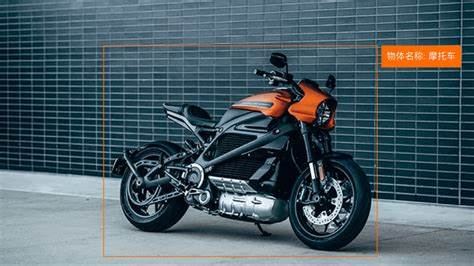
\includegraphics[width=0.9\columnwidth]{image/object_detection_examples.png} % 建议宽度
                %\centering \framebox[0.9\columnwidth][c]{示例图片区域} % 占位符
                \caption{目标检测应用示例}
            \end{figure}
        \end{column}
    \end{columns}
    
    \vspace{0.5cm}
    \begin{block}{技术挑战与我的思考}
        \begin{itemize}
            \item 精确的边界框定位
            \item 小目标和密集目标检测
            \item 实时性能与计算效率的平衡
            \item \textcolor{red}{思考：这些挑战中，哪一点最具突破性价值？为什么？}
        \end{itemize}
    \end{block}
\end{frame}

\section{四篇经典论文串讲与个人解读}
\subsection{R-CNN: Regions with Convolutional Neural Networks}
\begin{frame}{R-CNN (2014) - 开创先河}
    \begin{block}{核心贡献与历史地位}
        \begin{itemize}
            \item 首次将CNN引入目标检测领域
            \item 提出"区域建议+分类"的两阶段框架
            \item \textcolor{red}{我的理解：R-CNN的出现，其最大的历史意义是什么？它如何改变了后续目标检测的研究范式？}
        \end{itemize}
    \end{block}
    
    \begin{columns}[T]
        \begin{column}{0.48\textwidth}
            \textbf{工作流程}:
            \begin{enumerate}
                \item 使用Selective Search生成约2000个区域建议
                \item 对每个区域进行CNN特征提取 (AlexNet/VGG)
                \item 使用SVM进行分类
                \item 用边界框回归微调框位置
            \end{enumerate}
        \end{column}
        \hfill
        \begin{column}{0.48\textwidth}
            \begin{itemize}
                \item \textcolor{red}{思考：R-CNN的多阶段训练流程有什么优缺点？}
                \item \textcolor{red}{对比：与现代端到端模型相比，R-CNN的架构有哪些局限性？}
            \end{itemize}
        \end{column}
    \end{columns}
\end{frame}

\begin{frame}{R-CNN架构}
            \begin{figure}
                 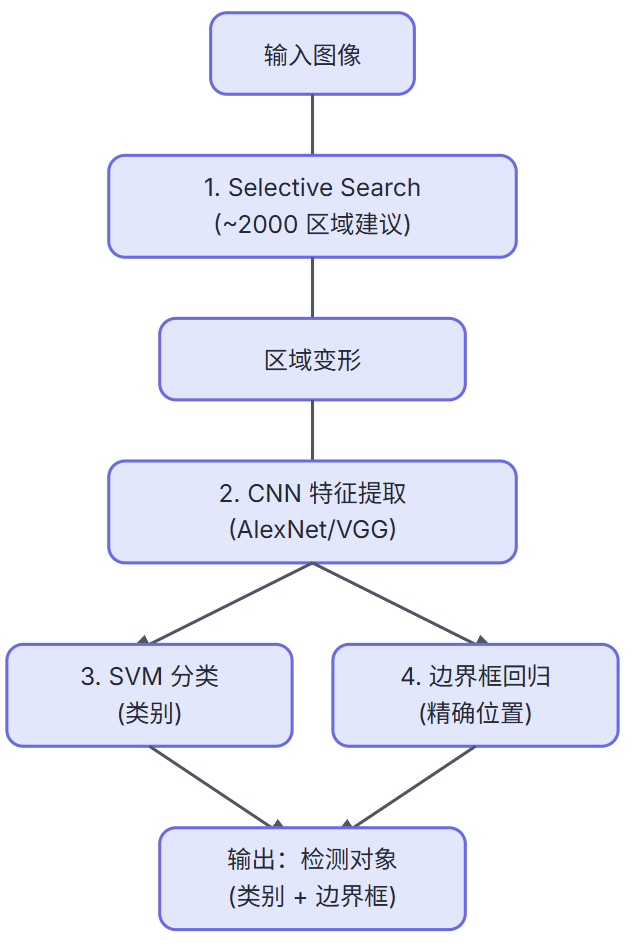
\includegraphics[width=0.4\columnwidth]{image/rcnn_architecture.png} % 建议宽度
                %\centering \framebox[0.9\columnwidth][c]{示例图片区域} % 占位符
                \caption{R-CNN架构}
            \end{figure}
\end{frame}

\begin{frame}{R-CNN 优缺点}
    \begin{columns}[T] % T 选项使列顶部对齐
        \begin{column}{0.48\textwidth}
            \begin{block}{优点}
                \begin{itemize}
                    \item 首次证明CNN用于目标检测的有效性
                    \item 模块化设计，易于理解和实现
                    \item 在PASCAL VOC上取得突破性结果
                \end{itemize}
            \end{block}
        \end{column}
        \hfill % 在两列之间添加弹性空间
        \begin{column}{0.48\textwidth}
            \begin{block}{局限性}
                \begin{itemize}
                    \item 训练过程繁琐且耗时
                    \item 检测速度慢 (每张图像约47秒)
                    \item 特征不共享，计算效率低
                \end{itemize}
            \end{block}
        \end{column}
    \end{columns}
\end{frame}

\begin{frame}{R-CNN实验结果与解读}
    \begin{table}
        \centering
        \caption{PASCAL VOC 2007测试集上的性能}
        \begin{tabular}{lcc}
            \toprule
            方法 & mAP (\%) & 每张图像耗时 (s) \\
            \midrule
            SIFT+HOG & 35.1 & - \\
            R-CNN (AlexNet) & 58.5 & 47 \\
            R-CNN (VGG16) & 66.0 & 82 \\
            \bottomrule
        \end{tabular}
    \end{table}
    
    \begin{itemize}
        \item 首次证明了CNN在目标检测中的有效性，mAP大幅提升
        \item 但计算效率成为实际应用的瓶颈
        \item \textcolor{red}{我的解读：从实验结果看，VGG16相较于AlexNet带来了精度提升，但也增加了耗时。这反映了当时深度模型在精度与效率间的权衡。如何看待这种权衡在当时的重要性？}
    \end{itemize}
\end{frame}

\subsection{Fast R-CNN - 效率的飞跃}
\begin{frame}{Fast R-CNN (2015)}
    \begin{block}{核心改进与思想}
        \begin{itemize}
            \item 提出RoI (Region of Interest)池化层，实现特征共享
            \item 统一的多任务损失函数 (分类 + 边界框回归)
            \item 单阶段训练过程 (除区域建议外)
            \item \textcolor{red}{我的理解：Fast R-CNN是如何巧妙地解决R-CNN效率瓶颈的？RoI池化的核心思想是什么？}
        \end{itemize}
    \end{block}
    
    \begin{columns}
        \begin{column}{0.5\textwidth}
            \textbf{关键创新}:
            \begin{itemize}
                \item 共享卷积计算：整张图像只通过CNN一次提取特征图
                \item RoI池化：将特征图上任意大小的区域建议映射到固定尺寸的特征向量
                \item 端到端联合训练分类器和边界框回归器
            \end{itemize}
        \end{column}
        \begin{column}{0.5\textwidth}
            \begin{figure}
                 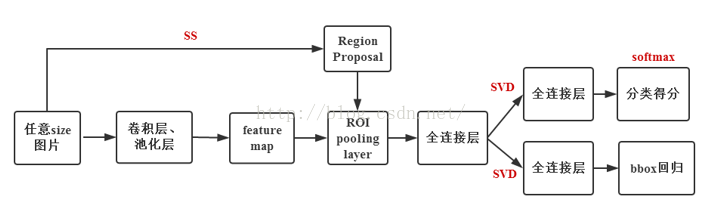
\includegraphics[width=0.9\columnwidth]{image/fast_rcnn_architecture.png} % 建议宽度
                %\centering \framebox[0.9\columnwidth][c]{Fast R-CNN架构图区域} % 占位符
                \caption{Fast R-CNN架构}
            \end{figure}
        \end{column}
    \end{columns}
\end{frame}

\begin{frame}{RoI池化层详解与思考}
    \begin{columns}
        \begin{column}{0.6\textwidth}
            \begin{itemize}
                \item 将特征图上的任意RoI映射为固定大小的特征向量
                \item 操作步骤：
                \begin{enumerate}
                    \item 将RoI投影到特征图
                    \item 将投影后的RoI划分为固定数量 (e.g., $H \times W$) 的子区域 (bins)
                    \item 对每个子区域执行max pooling
                \end{enumerate}
                \item 数学表达（示意）：
                \[
                \text{RoIPooling}(x,y)_{\text{bin}} = \max_{(i,j) \in \text{bin}(x,y)} \text{feature\_map}_{i,j}
                \]
                \item \textcolor{red}{我的理解：RoI池化层在Fast R-CNN乃至后续模型中的关键作用是什么？它如何实现对不同尺寸输入的统一处理？}
            \end{itemize}
        \end{column}
        \begin{column}{0.4\textwidth}
            \begin{figure}
                 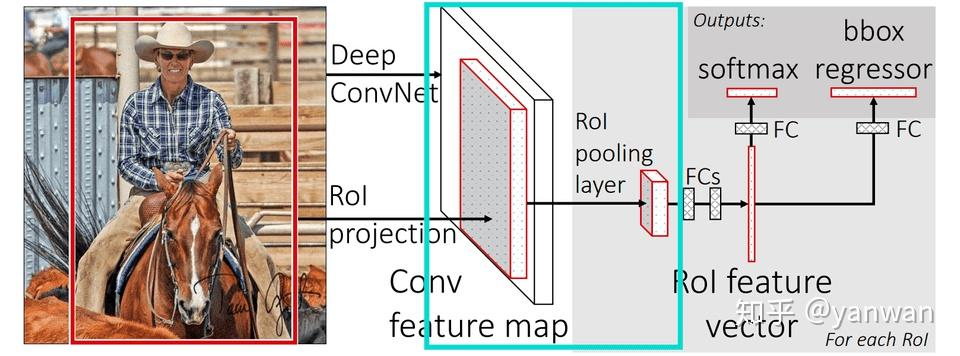
\includegraphics[width=0.9\columnwidth]{image/roi_pooling.png} % 建议宽度
                %\centering \framebox[0.9\columnwidth][c]{RoI池化示意图区域} % 占位符
                \caption{RoI池化操作}
            \end{figure}
        \end{column}
    \end{columns}
\end{frame}

\begin{frame}{Fast R-CNN实验结果与分析}
    \begin{table}
        \centering
        \caption{PASCAL VOC 2012测试集上的性能 (对比R-CNN)}
        \begin{tabular}{lcc}
            \toprule
            方法 & mAP (\%) & 每张图像耗时 (s) \\
            \midrule
            R-CNN (VGG16) & 66.0 & 82 \\ % VOC07数据，仅为对比示意
            Fast R-CNN (VGG16) & 70.0 & 2.3 (含Selective Search) \\
            \bottomrule
        \end{tabular}
    \end{table}
    
    \begin{itemize}
        \item 相比R-CNN，检测速度大幅提升 (训练速度提升约9倍，测试速度提升约10-100倍，不含区域建议)
        \item 端到端训练框架简化了模型流程，mAP也有所提升
        \item \textcolor{red}{我的分析：速度的巨大提升主要归功于哪些设计？Selective Search仍然是瓶颈，这暗示了什么？}
    \end{itemize}
\end{frame}

\subsection{Faster R-CNN - 迈向实时}
% 修改：拆分原Frame 10和Frame 11
\begin{frame}{Faster R-CNN (2015) - 核心思想}
    \begin{block}{核心贡献与突破}
        \begin{itemize}
            \item 提出区域建议网络 (Region Proposal Network, RPN)，替代Selective Search
            \item 实现近乎实时的端到端目标检测系统 (RPN与检测网络共享卷积特征)
            \item 引入锚点 (anchor) 机制，高效生成多尺度、多长宽比的候选框
            \item \textcolor{red}{我的理解：RPN的引入是怎样一个里程碑式的改进？它如何将区域建议也纳入到神经网络中进行学习？}
        \end{itemize}
    \end{block}
\end{frame}
\begin{frame}{Faster R-CNN架构图}
        \begin{center}
        \begin{figure}
             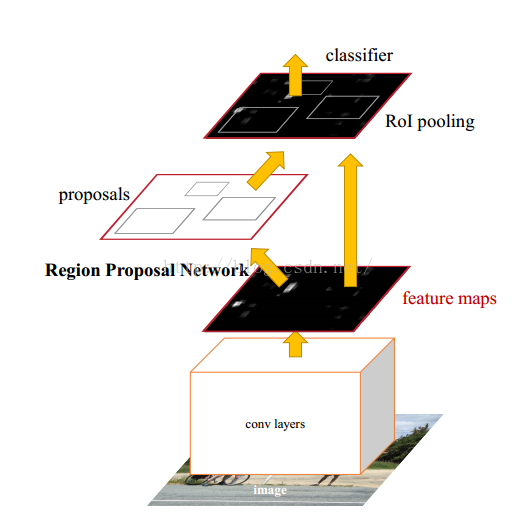
\includegraphics[width=0.5\textwidth]{image/faster_rcnn_architecture.png} % 建议宽度
            %\centering \framebox[0.7\textwidth][c]{Faster R-CNN整体架构图区域} % 占位符
            \caption{Faster R-CNN整体架构}
        \end{figure}
    \end{center}
\end{frame}


\begin{frame}[fragile]{区域建议网络(RPN)详解}
    \begin{columns}
        \begin{column}{0.6\textwidth}
            \textbf{RPN工作原理}:
            \begin{itemize}
                \item RPN是一个全卷积网络，在主干网络输出的特征图上滑动窗口
                \item 每个滑动窗口中心位置，与一组预设的锚点 (anchors) 关联
                \item RPN通过两个并行的全连接层（实现为1x1卷积）输出：
                    \begin{itemize}
                        \item 每个锚点是否为目标的得分 (objectness score)
                        \item 每个锚点的边界框回归偏移量 (bounding box regression)
                    \end{itemize}
                \item 与检测网络共享卷积特征，计算成本低
            \end{itemize}
        \end{column}
        \begin{column}{0.4\textwidth}
            \begin{figure}
                 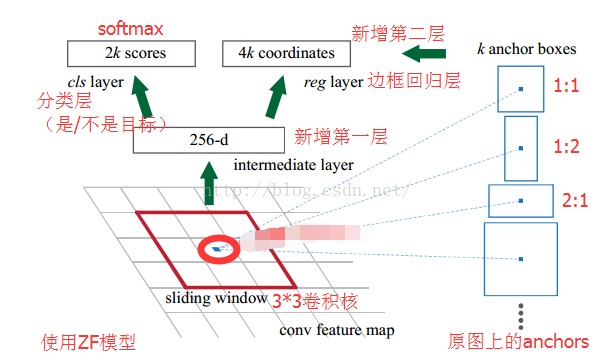
\includegraphics[width=\columnwidth]{image/rpn_architecture.png} % 建议宽度
                %\centering \framebox[0.9\columnwidth][c]{RPN架构图区域} % 占位符
                \caption{RPN架构}
            \end{figure}
        \end{column}
    \end{columns}
\end{frame}

\begin{frame}[fragile]{锚点(Anchor)机制解析}
    \textbf{锚点机制}:
    \begin{itemize}
        \item 在特征图的每个空间位置，预设k个具有不同尺度 (scales) 和长宽比 (aspect ratios) 的参考框（锚点）。
        \item 例如，常用的设置为3种尺度和3种长宽比，即每个位置9个锚点。
        \item RPN的任务是判断这些锚点中哪些包含目标，并对它们的位置进行微调。
        \item \textcolor{red}{我的思考：锚点机制的设计有何巧妙之处？它如何有效地覆盖图像中各种形状和大小的目标？相比于传统的滑动窗口方法有何优势？}
    \end{itemize}
    \begin{center}
        \begin{figure}
             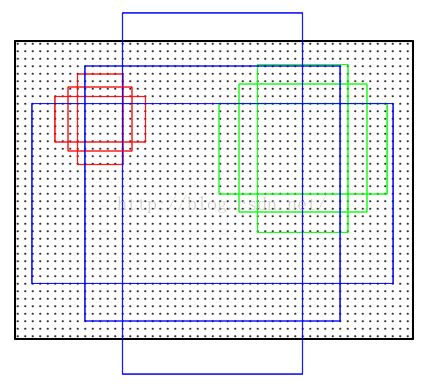
\includegraphics[width=0.2\textwidth]{image/anchors.png} % 建议宽度
            % \centering \framebox[0.6\textwidth][c]{锚点示意图区域} % 占位符
            \caption{不同尺度和宽高比的锚点示例}
        \end{figure}
    \end{center}
\end{frame}


\begin{frame}{Faster R-CNN实验结果与意义}




\begin{table}
    \centering
    \caption{MS COCO 2015测试集上的性能 (对比Fast R-CNN)}
    \resizebox{\textwidth}{!}{ % 自动缩放表格宽度
        \begin{tabular}{@{}lccc@{}}
            \toprule
            方法 & \multicolumn{1}{c}{mAP@.5 (\%)} & \multicolumn{1}{c}{mAP@[.5:.95] (\%)} & \multicolumn{1}{c}{速度 (fps, VGG16)} \\
            \midrule
            Fast R-CNN (SS) & 39.3 & 19.7 & 0.5 \\
            Faster R-CNN (RPN) & 42.7 & 21.9 & 5-7 \\
            \bottomrule
        \end{tabular}
    }
\end{table}
    
    \begin{itemize}
        \item RPN网络显著提升了区域建议的质量和速度，几乎不增加额外计算量
        \item 首次实现了接近实时的两阶段目标检测 (如用ZFNet可达17fps)
        \item \textcolor{red}{我的解读：Faster R-CNN的成功对后续的目标检测算法（包括单阶段检测器）有何启发和影响？}
    \end{itemize}
\end{frame}

\subsection{Mask R-CNN - 拓展至实例分割}
\begin{frame}{Mask R-CNN (2017)}
    \begin{block}{核心贡献与创新点}
        \begin{itemize}
            \item 扩展Faster R-CNN，在检测边界框的同时，实现像素级的实例分割
            \item 提出RoIAlign替代RoIPooling，解决特征错位问题，提升分割精度
            \item 并行预测类别、边界框和分割掩码 (mask)
            \item \textcolor{red}{我的理解：从目标检测到实例分割，Mask R-CNN是如何优雅地扩展Faster R-CNN框架并解决关键挑战的？}
        \end{itemize}
    \end{block}
\end{frame}
\begin{frame}{Mask R-CNN 架构}
        \begin{center}
        \begin{figure}
             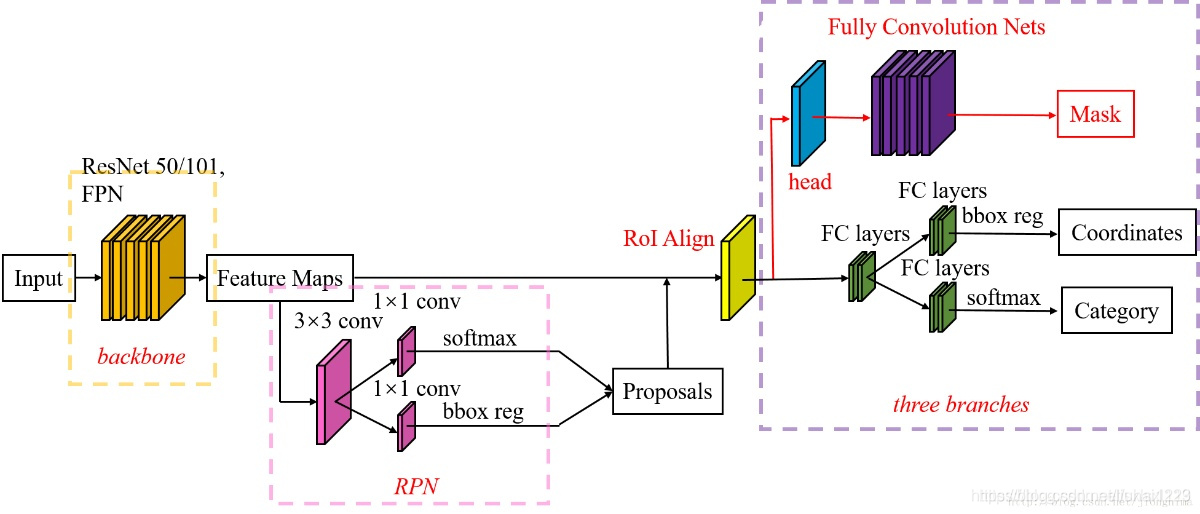
\includegraphics[width=1\textwidth]{image/mask_rcnn_architecture.png} % 建议宽度
            %\centering \framebox[0.65\textwidth][c]{Mask R-CNN架构图区域} % 占位符
            \caption{Mask R-CNN架构}
        \end{figure}
    \end{center}
\end{frame}

\begin{frame}[fragile]{RoIAlign vs RoIPooling - 精度的关键} % 添加[fragile]
    \begin{columns}
        \begin{column}{0.5\textwidth}
            \textbf{RoIPooling的问题}:
            \begin{itemize}
                \item 两次量化操作 (取整) 导致候选区域特征与原图不对齐 (misalignment)
                \item 这种不对齐对分类任务影响较小，但对像素级的分割掩码精度影响较大
            \end{itemize}
            
            \begin{figure}
                 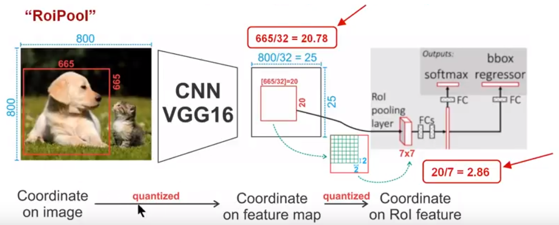
\includegraphics[width=0.8\columnwidth]{image/roipooling_problem.png} % 建议宽度
                %\centering \framebox[0.9\columnwidth][c]{RoIPooling量化问题示意图} % 占位符
                \caption{RoIPooling的量化问题}
            \end{figure}
        \end{column}
        \begin{column}{0.5\textwidth}
            \textbf{RoIAlign的改进}:
            \begin{itemize}
                \item 避免任何量化操作，保持浮点坐标
                \item 使用双线性插值 (bilinear interpolation) 在每个RoI bin的采样点上计算精确的特征值
                \item 保持特征与原图的严格对齐关系
                \item \textcolor{red}{我的理解：RoIAlign为何能显著提升分割精度？其核心思想“对齐”体现在哪里？}
            \end{itemize}
            
            \begin{figure}
                 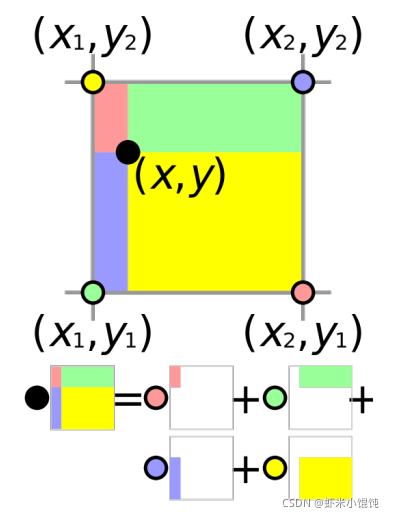
\includegraphics[width=0.1\columnwidth]{image/roialign.png} % 建议宽度
                %\centering \framebox[0.9\columnwidth][c]{RoIAlign双线性插值示意图} % 占位符
                \caption{RoIAlign的双线性插值}
            \end{figure}
        \end{column}
    \end{columns}
\end{frame}

\begin{frame}{Mask R-CNN实验结果与价值}
    \begin{table}
        \centering
        \caption{COCO 2017测试集上的性能}
        \begin{tabular}{lcccc}
            \toprule
            方法 & 检测mAP & 分割mAP & 小目标AP & 推理速度 (fps) \\ 
            \midrule
            Faster R-CNN & 35.9 & - & 16.8 & 5.0 \\ % 示例数据
            Mask R-CNN & 38.2 & 34.8 & 18.3 & 5.0 \\ % 示例数据
            \bottomrule
        \end{tabular}
    \end{table}
    
    \begin{itemize}
        \item 在不显著牺牲检测速度的前提下，实现了高质量的实例分割
        \item RoIAlign对分割精度的提升作用显著，尤其在小目标和边缘区域
        \item Mask R-CNN成为后续许多实例分割、关键点检测等任务的基础框架
        \item \textcolor{red}{我的评价：Mask R-CNN的通用性和强大性能使其成为计算机视觉领域的里程碑之作。对后续多任务学习有何启示？}
    \end{itemize}
\end{frame}
\begin{frame}[fragile]{四篇论文的演进脉络与我的洞察}
    \begin{center}
        \resizebox{\textwidth}{!}{ % 自动调整大小以适应页面宽度
        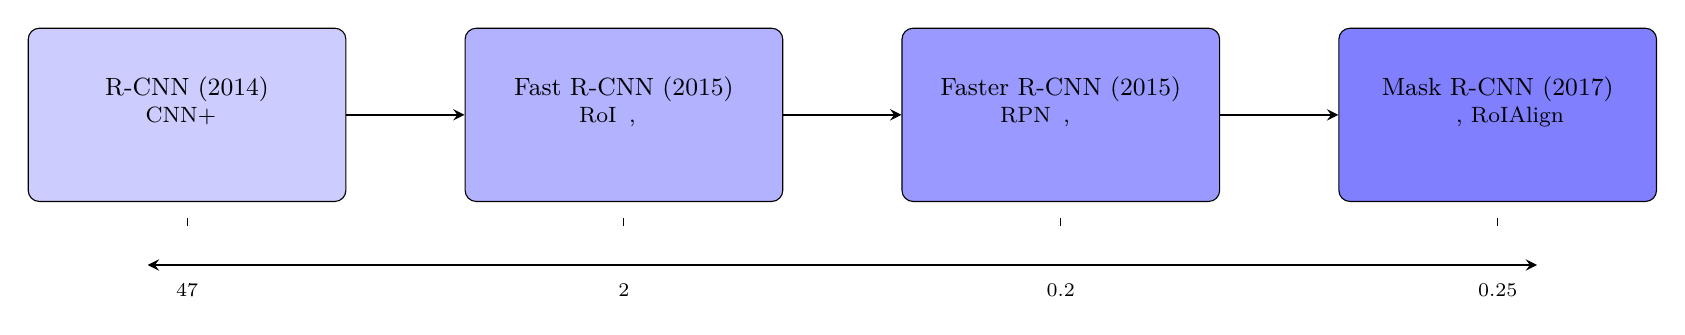
\begin{tikzpicture}[
            node distance=1.5cm, % 节点间距
            rect/.style={rectangle, draw, fill=blue!20, text width=3.8cm, text centered, rounded corners, minimum height=2.2cm, font=\small}, % 调整文本宽度和字体
            arrow/.style={thick, ->, >=stealth},
            annotation/.style={text width=3cm, align=center, font=\scriptsize} % 注释样式
        ]
        
        % 定义节点
        \node (rcnn) [rect] {R-CNN (2014)\\ \footnotesize 首次CNN+区域建议\\奠定基础};
        \node (fast) [rect, fill=blue!30, right=of rcnn] {Fast R-CNN (2015)\\ \footnotesize RoI池化, 特征共享\\提升效率};
        \node (faster) [rect, fill=blue!40, right=of fast] {Faster R-CNN (2015)\\ \footnotesize RPN网络, 端到端区域建议\\迈向实时};
        \node (mask) [rect, fill=blue!50, right=of faster] {Mask R-CNN (2017)\\ \footnotesize 实例分割, RoIAlign\\拓展功能};
        
        % 连接线和演进注释
        \draw [arrow] (rcnn.east) -- (fast.west) 
            node[midway, above, yshift=0.3cm, annotation] {\textcolor{red}{\scriptsize 解决效率问题}};
        \draw [arrow] (fast.east) -- (faster.west) 
            node[midway, above, yshift=0.3cm, annotation] {\textcolor{red}{\scriptsize 解决速度瓶颈}};
        \draw [arrow] (faster.east) -- (mask.west) 
            node[midway, above, yshift=0.3cm, annotation] {\textcolor{red}{\scriptsize 拓展任务范畴}};
        
        % 性能对比注释
        \node[below=0.8cm of rcnn, annotation] {\scriptsize 每张图像\\约47秒};
        \node[below=0.8cm of fast, annotation] {\scriptsize 每张图像\\约2秒};
        \node[below=0.8cm of faster, annotation] {\scriptsize 每张图像\\约0.2秒};
        \node[below=0.8cm of mask, annotation] {\scriptsize 每张图像\\约0.25秒};
        
        % 垂直连接线
        \draw[dashed, shorten >=0.2cm, shorten <=0.2cm] (rcnn.south) -- ++(0,-0.6cm);
        \draw[dashed, shorten >=0.2cm, shorten <=0.2cm] (fast.south) -- ++(0,-0.6cm);
        \draw[dashed, shorten >=0.2cm, shorten <=0.2cm] (faster.south) -- ++(0,-0.6cm);
        \draw[dashed, shorten >=0.2cm, shorten <=0.2cm] (mask.south) -- ++(0,-0.6cm);
        
        % 演进趋势箭头
        \draw[thick, <->, >=stealth] ([xshift=-0.5cm, yshift=-0.8cm]rcnn.south) -- ([xshift=0.5cm, yshift=-0.8cm]mask.south)
            node[midway, below, yshift=-0.2cm] {\Large \textbf{性能提升}};
        
        \end{tikzpicture}
        }
    \end{center}
    
    \begin{itemize}
        \item 计算效率不断提升: 从R-CNN的分钟级到Mask R-CNN的接近实时
        \item 功能不断扩展: 从单纯检测到实例分割，乃至更多任务
        \item 架构不断优化: 从多阶段繁琐训练到端到端联合训练
        \item \textcolor{red}{我的洞察：这一系列演进体现了科研中哪些重要的思想？例如问题驱动、逐步优化、模块化设计等。您从中获得了哪些启发？}
    \end{itemize}
\end{frame}

\begin{frame}[fragile]{性能对比总结与深层解读} % 添加[fragile]
    \begin{center} % 使图表居中
    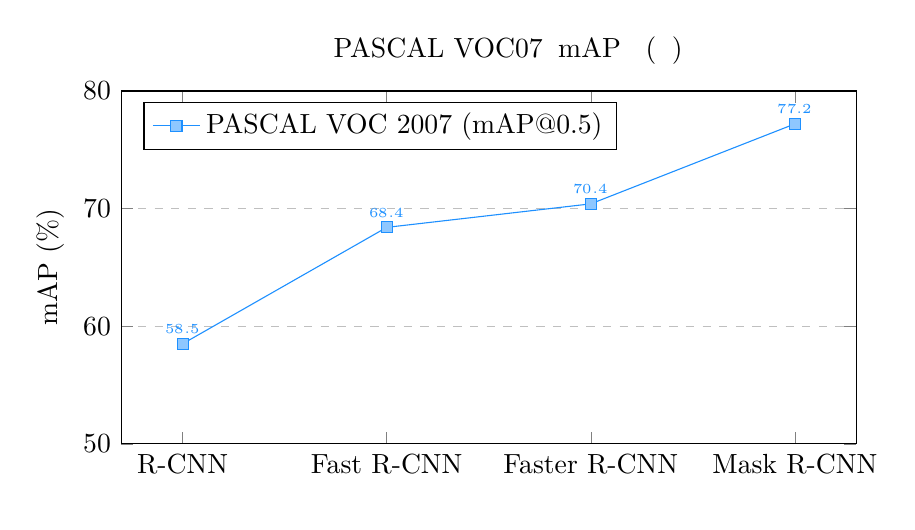
\begin{tikzpicture}
        \begin{axis}[
            width=0.9\textwidth, % 修改：调整图表宽度
            height=0.5\textwidth, % 修改：调整图表高度
            title={四篇论文在PASCAL VOC07上的mAP对比 (示意)},
            xlabel={方法},
            ylabel={mAP (\%)},
            ymin=50, ymax=80,
            symbolic x coords={R-CNN,Fast R-CNN,Faster R-CNN,Mask R-CNN},
            xtick=data,
            nodes near coords,
            nodes near coords style={font=\tiny}, % 减小nodes near coords字体
            nodes near coords align={vertical},
            legend pos=north west,
            ymajorgrids=true,
            grid style=dashed,
        ]
        \addplot[color=myblue,mark=square*, mark options={fill=myblue!50}] coordinates {
            (R-CNN,58.5) 
            (Fast R-CNN,68.4) 
            (Faster R-CNN,70.4) 
            (Mask R-CNN,77.2) 
        };
        \addlegendentry{PASCAL VOC 2007 (mAP@0.5)}
        \end{axis}
    \end{tikzpicture}
    \end{center}
    \begin{itemize}
        \item \textcolor{red}{我的解读：这张图直观地展示了性能的提升。但除了数字本身，还能从中解读出哪些信息？例如，性能提升的幅度在后期是否趋缓？这可能意味着什么？}
    \end{itemize}
\end{frame}
\section{新芽讲座学习心得与个人思考}
\begin{frame}{新芽讲座学习心得}
    \begin{block}{讲座主题}
        "面向复杂PC任务的多模态智能体框架" - 张熙 (2025)
    \end{block}
    
    \begin{columns}
        \begin{column}{0.6\textwidth}
            \begin{itemize}
                \item 学习收获:
                \begin{itemize}
                    \item 理解大模型智能体的核心优势：知识丰富性、推理规划能力、工具使用能力
                    \item 掌握多模态智能体的三大应用赛道：助手效率型、个性化、多模态
                    \item 了解PC Agent面临的核心挑战及解决方案
                \end{itemize}
            \end{itemize}
        \end{column}
        \begin{column}{0.4\textwidth}
            \begin{figure}
                %\includegraphics[width=\textwidth]{multimodal_agent.png}
                %\caption{多模态智能体框架}
            \end{figure}
        \end{column}
    \end{columns}
\end{frame}

\begin{frame}{PC Agent的核心挑战与解决方案}
    \begin{columns}[T] % 使用[T]确保顶部对齐
        \begin{column}{0.49\textwidth} % 精确控制列宽
            \begin{block}{感知难点与解决思路}
                \begin{itemize}
                    \item<1-> \textbf{难点：}
                    \begin{itemize}
                        \item PC屏幕大，交互元素密集多样
                        \item 文本布局复杂，模型理解困难
                    \end{itemize}
                    \item<2-> \textbf{解决方法：}
                    \begin{itemize}
                        \item 使用AIA Eleven y tree提取可交互元素
                        \item 引入主动感知模块处理文本
                    \end{itemize}
                \end{itemize}
            \end{block}
        \end{column}
        \hfill % 在两列之间添加弹性空间
        \begin{column}{0.49\textwidth} % 精确控制列宽
            \begin{block}{决策难点与解决思路}
                \begin{itemize}
                    \item<1-> \textbf{难点：}
                    \begin{itemize}
                        \item 用户指令包含复杂操作序列
                        \item 涉及更多复杂APP和跨APP工作流
                    \end{itemize}
                    \item<2-> \textbf{解决方法：}
                    \begin{itemize}
                        \item 将指令拆分为指令、子任务、动作三个层级
                        \item 引入manager agent、progress agent、decision agent和reflection agent
                    \end{itemize}
                \end{itemize}
            \end{block}
        \end{column}
    \end{columns}
    
    % 可选：添加底部说明
    \vspace{0.3cm}
    \begin{center}
        \textcolor{gray}{\footnotesize 注：两个模块协同工作，实现PC端复杂任务的自动化处理}
    \end{center}
\end{frame}

\begin{frame}{开源应用与热点探讨}
    \begin{block}{开源应用}
        \begin{itemize}
            \item Mobile Agent: 支持手机端复杂任务自动化
            \item PC Agent: 支持桌面应用复杂交互
            \item 开源框架特点：模块化设计、可扩展性强
        \end{itemize}
    \end{block}
    
    \begin{block}{热点与未来方向}
        \begin{itemize}
            \item 热点：deep research、menus、open menus
            \item 未来方向：
            \begin{itemize}
                \item 更通用泛化的执行方式
                \item 多模态内容理解与生成
                \item 增强长期记忆与推理能力
                \item 提升跨应用工作流效率
            \end{itemize}
        \end{itemize}
    \end{block}
\end{frame}

\begin{frame}{互动问答与个人思考}
    \begin{block}{关键问答}
        \begin{itemize}
            \item 关于PK线加入语言交互计划：正在研发中，计划Q3推出预览版
            \item 数据安全保证：采用端到端加密和联邦学习技术
            \item 基座大模型选择：根据具体任务选择最适合的模型架构
            \item agent设计流程：模块化设计，强调可解释性和可控性
            \item 多模态数据处理：融合文本、视觉和交互信号
        \end{itemize}
    \end{block}
    

\end{frame}

\section{总结与展望}
\begin{frame}{总结}
    \begin{block}{技术演进总结与启示}
        \begin{itemize}
            \item 两阶段检测框架从R-CNN到Mask R-CNN的演进是目标检测领域的重要里程碑，清晰地展现了问题驱动的技术发展路径。
            \item 每篇论文都针对前作的不足提出了创新性解决方案，推动了整个领域的前进。
            \item 这些技术不仅在学术界影响深远，也为工业界的广泛应用奠定了坚实基础。
            %\item \textcolor{red}{我的总结：回顾这段技术史，最让您印象深刻的创新点是什么？它体现了怎样的科研智慧？}
        \end{itemize}
    \end{block}
\end{frame}
% \begin{frame}{总结、展望与个人规划}
%     \begin{block}{未来方向与个人关注}
%         \begin{itemize}
%             \item 提升小目标、遮挡、密集目标的检测性能依然是重点。
%             \item 探索更高效、更轻量级的检测架构，以适应边缘计算和移动设备的需求。
%             \item 结合多模态信息 (如文本、音频) 和上下文理解，提升检测的鲁棒性和智能化水平。
%             \item 研究开放世界、持续学习环境下的目标检测，使模型能适应动态变化的环境。
%             \item \textcolor{red}{我特别关注的未来方向：[请在此处阐述您最感兴趣的1-2个未来方向，并说明原因及其潜在价值]}
%         \end{itemize}
%     \end{block}
% \end{frame}

% % 修改：拆分原Frame 24
% \begin{frame}{我的研究计划与思考}
%     \begin{itemize}
%         \item \textbf{方向一：} 基于Transformer架构改进目标检测模型
%             \begin{itemize}
%                 \item \textcolor{red}{阐述：为何选择Transformer？预期它能解决当前检测模型的哪些问题？初步的技术方案是什么？}
%             \end{itemize}
%             \vspace{0.5em} % 增加条目间距
%         \item \textbf{方向二：} 探索目标检测在医学图像分析 (如肿瘤检测、病灶分割) 中的应用
%             \begin{itemize}
%                 \item \textcolor{red}{阐述：该应用场景的特殊性和挑战性是什么？目标检测技术能带来哪些价值？}
%             \end{itemize}
%             \vspace{0.5em}
%         \item \textbf{方向三：} 研究模型压缩和量化技术，实现高效的边缘设备部署
%             \begin{itemize}
%                 \item \textcolor{red}{阐述：针对特定应用场景，对模型大小和速度有何要求？计划采用哪些压缩或量化策略？}
%             \end{itemize}
%     \end{itemize}
% \end{frame}

% \begin{frame}{初步实验结果与分析}
%     \begin{block}{初步实验结果与分析 (若有)}
%         \begin{itemize}
%             \item 示例：在医学超声图像数据集上，改进的Faster R-CNN模型初步实现了82.3\%的mAP。
%                 \begin{itemize}
%                     \item \textcolor{red}{分析：这一结果达到了怎样的水平？对比基线模型有何提升？实验中遇到了哪些挑战？下一步的优化方向是什么？}
%                 \end{itemize}
%                 \vspace{0.5em}
%             \item 示例：通过知识蒸馏，模型大小压缩了75\%，推理速度在特定硬件上提升3倍，精度损失控制在2\%以内。
%                 \begin{itemize}
%                     \item \textcolor{red}{分析：压缩效果是否达到预期？精度与效率的权衡如何？对实际部署有何意义？}
%                 \end{itemize}
%         \end{itemize}
%     \end{block}
% \end{frame}


% 问答页
\begin{frame}{Questions and Answers}
  \centering
  \vspace{0.8cm}
  {\Huge \bfseries Q\&A}
\end{frame}

\begin{frame}[allowframebreaks]{参考文献}
    \bibliographystyle{apalike} 
    % \bibliography{references} 

    \begin{thebibliography}{99}
        \bibitem{girshick2014rcnn}
        Girshick, R., Donahue, J., Darrell, T., \& Malik, J. (2014). Rich feature hierarchies for accurate object detection and semantic segmentation. In \textit{Proceedings of the IEEE conference on computer vision and pattern recognition} (pp. 580-587).
        
        \bibitem{girshick2015fast}
        Girshick, R. (2015). Fast r-cnn. In \textit{Proceedings of the IEEE international conference on computer vision} (pp. 1440-1448).
        
        \bibitem{ren2015faster}
        Ren, S., He, K., Girshick, R., \& Sun, J. (2015). Faster r-cnn: Towards real-time object detection with region proposal networks. \textit{Advances in neural information processing systems}, 28.
        
        \bibitem{he2017mask}
        He, K., Gkioxari, G., Dollár, P., \& Girshick, R. (2017). Mask r-cnn. In \textit{Proceedings of the IEEE international conference on computer vision} (pp. 2961-2969).
        \bibitem{newsprout2025}
        张熙, 算法工程师. (2025). 面向复杂PC任务的多模态智能体框架. 青稞Talk 41.


    \end{thebibliography}
\end{frame}

%结束页
\begin{frame}[plain]
  \begin{tikzpicture}[remember picture,overlay]
    % 背景设置：使用深蓝色半透明背景
    \node[fill=midblue, opacity=1, minimum width=\paperwidth, minimum height=\paperheight] at (current page.center) {};
    % THANKS 文本设置：白色大字号
    \node[font=\fontsize{40}{70}\selectfont\bfseries, text=white] at (current page.center) {THANKS};
  \end{tikzpicture}
\end{frame}

\end{document}
